\documentclass[1p]{elsarticle_modified}
%\bibliographystyle{elsarticle-num}

%\usepackage[colorlinks]{hyperref}
%\usepackage{abbrmath_seonhwa} %\Abb, \Ascr, \Acal ,\Abf, \Afrak
\usepackage{amsfonts}
\usepackage{amssymb}
\usepackage{amsmath}
\usepackage{amsthm}
\usepackage{scalefnt}
\usepackage{amsbsy}
\usepackage{kotex}
\usepackage{caption}
\usepackage{subfig}
\usepackage{color}
\usepackage{graphicx}
\usepackage{xcolor} %% white, black, red, green, blue, cyan, magenta, yellow
\usepackage{float}
\usepackage{setspace}
\usepackage{hyperref}

\usepackage{tikz}
\usetikzlibrary{arrows}

\usepackage{multirow}
\usepackage{array} % fixed length table
\usepackage{hhline}

%%%%%%%%%%%%%%%%%%%%%
\makeatletter
\renewcommand*\env@matrix[1][\arraystretch]{%
	\edef\arraystretch{#1}%
	\hskip -\arraycolsep
	\let\@ifnextchar\new@ifnextchar
	\array{*\c@MaxMatrixCols c}}
\makeatother %https://tex.stackexchange.com/questions/14071/how-can-i-increase-the-line-spacing-in-a-matrix
%%%%%%%%%%%%%%%

\usepackage[normalem]{ulem}

\newcommand{\msout}[1]{\ifmmode\text{\sout{\ensuremath{#1}}}\else\sout{#1}\fi}
%SOURCE: \msout is \stkout macro in https://tex.stackexchange.com/questions/20609/strikeout-in-math-mode

\newcommand{\cancel}[1]{
	\ifmmode
	{\color{red}\msout{#1}}
	\else
	{\color{red}\sout{#1}}
	\fi
}

\newcommand{\add}[1]{
	{\color{blue}\uwave{#1}}
}

\newcommand{\replace}[2]{
	\ifmmode
	{\color{red}\msout{#1}}{\color{blue}\uwave{#2}}
	\else
	{\color{red}\sout{#1}}{\color{blue}\uwave{#2}}
	\fi
}

\newcommand{\Sol}{\mathcal{S}} %segment
\newcommand{\D}{D} %diagram
\newcommand{\A}{\mathcal{A}} %arc


%%%%%%%%%%%%%%%%%%%%%%%%%%%%%5 test

\def\sl{\operatorname{\textup{SL}}(2,\Cbb)}
\def\psl{\operatorname{\textup{PSL}}(2,\Cbb)}
\def\quan{\mkern 1mu \triangleright \mkern 1mu}

\theoremstyle{definition}
\newtheorem{thm}{Theorem}[section]
\newtheorem{prop}[thm]{Proposition}
\newtheorem{lem}[thm]{Lemma}
\newtheorem{ques}[thm]{Question}
\newtheorem{cor}[thm]{Corollary}
\newtheorem{defn}[thm]{Definition}
\newtheorem{exam}[thm]{Example}
\newtheorem{rmk}[thm]{Remark}
\newtheorem{alg}[thm]{Algorithm}

\newcommand{\I}{\sqrt{-1}}
\begin{document}

%\begin{frontmatter}
%
%\title{Boundary parabolic representations of knots up to 8 crossings}
%
%%% Group authors per affiliation:
%\author{Yunhi Cho} 
%\address{Department of Mathematics, University of Seoul, Seoul, Korea}
%\ead{yhcho@uos.ac.kr}
%
%
%\author{Seonhwa Kim} %\fnref{s_kim}}
%\address{Center for Geometry and Physics, Institute for Basic Science, Pohang, 37673, Korea}
%\ead{ryeona17@ibs.re.kr}
%
%\author{Hyuk Kim}
%\address{Department of Mathematical Sciences, Seoul National University, Seoul 08826, Korea}
%\ead{hyukkim@snu.ac.kr}
%
%\author{Seokbeom Yoon}
%\address{Department of Mathematical Sciences, Seoul National University, Seoul, 08826,  Korea}
%\ead{sbyoon15@snu.ac.kr}
%
%\begin{abstract}
%We find all boundary parabolic representation of knots up to 8 crossings.
%
%\end{abstract}
%\begin{keyword}
%    \MSC[2010] 57M25 
%\end{keyword}
%
%\end{frontmatter}

%\linenumbers
%\tableofcontents
%
\newcommand\colored[1]{\textcolor{white}{\rule[-0.35ex]{0.8em}{1.4ex}}\kern-0.8em\color{red} #1}%
%\newcommand\colored[1]{\textcolor{white}{ #1}\kern-2.17ex	\textcolor{white}{ #1}\kern-1.81ex	\textcolor{white}{ #1}\kern-2.15ex\color{red}#1	}

{\Large $\underline{12n_{0209}~(K12n_{0209})}$}

\setlength{\tabcolsep}{10pt}
\renewcommand{\arraystretch}{1.6}
\vspace{1cm}\begin{tabular}{m{100pt}>{\centering\arraybackslash}m{274pt}}
\multirow{5}{120pt}{
	\centering
	\includegraphics[width=112pt]{../../../GIT/diagram.site/Diagrams/png/2298_12n_0209.png}\\
\ \ \ A knot diagram\footnotemark}&
\allowdisplaybreaks
\textbf{Linearized knot diagam} \\
\cline{2-2}
 &
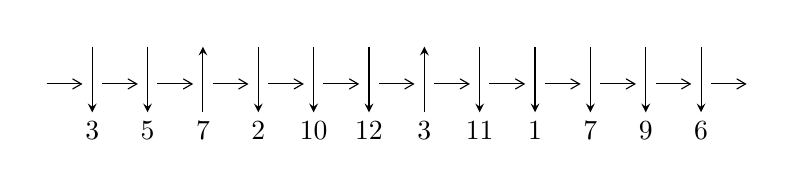
\begin{tikzpicture}[x=20pt, y=17pt]
	% nodes
	\node (C0) at (0, 0) {};
	\node (C1) at (1, 0) {};
	\node (C1U) at (1, +1) {};
	\node (C1D) at (1, -1) {3};

	\node (C2) at (2, 0) {};
	\node (C2U) at (2, +1) {};
	\node (C2D) at (2, -1) {5};

	\node (C3) at (3, 0) {};
	\node (C3U) at (3, +1) {};
	\node (C3D) at (3, -1) {7};

	\node (C4) at (4, 0) {};
	\node (C4U) at (4, +1) {};
	\node (C4D) at (4, -1) {2};

	\node (C5) at (5, 0) {};
	\node (C5U) at (5, +1) {};
	\node (C5D) at (5, -1) {10};

	\node (C6) at (6, 0) {};
	\node (C6U) at (6, +1) {};
	\node (C6D) at (6, -1) {12};

	\node (C7) at (7, 0) {};
	\node (C7U) at (7, +1) {};
	\node (C7D) at (7, -1) {3};

	\node (C8) at (8, 0) {};
	\node (C8U) at (8, +1) {};
	\node (C8D) at (8, -1) {11};

	\node (C9) at (9, 0) {};
	\node (C9U) at (9, +1) {};
	\node (C9D) at (9, -1) {1};

	\node (C10) at (10, 0) {};
	\node (C10U) at (10, +1) {};
	\node (C10D) at (10, -1) {7};

	\node (C11) at (11, 0) {};
	\node (C11U) at (11, +1) {};
	\node (C11D) at (11, -1) {9};

	\node (C12) at (12, 0) {};
	\node (C12U) at (12, +1) {};
	\node (C12D) at (12, -1) {6};
	\node (C13) at (13, 0) {};

	% arrows
	\draw[->,>={angle 60}]
	(C0) edge (C1) (C1) edge (C2) (C2) edge (C3) (C3) edge (C4) (C4) edge (C5) (C5) edge (C6) (C6) edge (C7) (C7) edge (C8) (C8) edge (C9) (C9) edge (C10) (C10) edge (C11) (C11) edge (C12) (C12) edge (C13) ;	\draw[->,>=stealth]
	(C1U) edge (C1D) (C2U) edge (C2D) (C3D) edge (C3U) (C4U) edge (C4D) (C5U) edge (C5D) (C6U) edge (C6D) (C7D) edge (C7U) (C8U) edge (C8D) (C9U) edge (C9D) (C10U) edge (C10D) (C11U) edge (C11D) (C12U) edge (C12D) ;
	\end{tikzpicture} \\
\hhline{~~} \\& 
\textbf{Solving Sequence} \\ \cline{2-2} 
 &
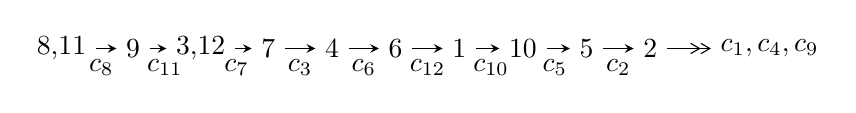
\begin{tikzpicture}[x=23pt, y=7pt]
	% node
	\node (A0) at (-1/8, 0) {8,11};
	\node (A1) at (1, 0) {9};
	\node (A2) at (33/16, 0) {3,12};
	\node (A3) at (25/8, 0) {7};
	\node (A4) at (33/8, 0) {4};
	\node (A5) at (41/8, 0) {6};
	\node (A6) at (49/8, 0) {1};
	\node (A7) at (57/8, 0) {10};
	\node (A8) at (65/8, 0) {5};
	\node (A9) at (73/8, 0) {2};
	\node (C1) at (1/2, -1) {$c_{8}$};
	\node (C2) at (3/2, -1) {$c_{11}$};
	\node (C3) at (21/8, -1) {$c_{7}$};
	\node (C4) at (29/8, -1) {$c_{3}$};
	\node (C5) at (37/8, -1) {$c_{6}$};
	\node (C6) at (45/8, -1) {$c_{12}$};
	\node (C7) at (53/8, -1) {$c_{10}$};
	\node (C8) at (61/8, -1) {$c_{5}$};
	\node (C9) at (69/8, -1) {$c_{2}$};
	\node (A10) at (11, 0) {$c_{1},c_{4},c_{9}$};

	% edge
	\draw[->,>=stealth]	
	(A0) edge (A1) (A1) edge (A2) (A2) edge (A3) (A3) edge (A4) (A4) edge (A5) (A5) edge (A6) (A6) edge (A7) (A7) edge (A8) (A8) edge (A9) ;
	\draw[->>,>={angle 60}]	
	(A9) edge (A10);
\end{tikzpicture} \\ 

\end{tabular} \\

\footnotetext{
The image of knot diagram is generated by the software ``\textbf{Draw programme}" developed by Andrew Bartholomew(\url{http://www.layer8.co.uk/maths/draw/index.htm\#Running-draw}), where we modified some parts for our purpose(\url{https://github.com/CATsTAILs/LinksPainter}).
}\phantom \\ \newline 
\centering \textbf{Ideals for irreducible components\footnotemark of $X_{\text{par}}$} 
 
\begin{align*}
I^u_{1}&=\langle 
-5.23422\times10^{225} u^{80}-3.14728\times10^{226} u^{79}+\cdots+7.26097\times10^{226} b-1.56109\times10^{228},\\
\phantom{I^u_{1}}&\phantom{= \langle  }1.52450\times10^{227} u^{80}+8.16205\times10^{227} u^{79}+\cdots+1.04921\times10^{229} a+3.18901\times10^{229},\\
\phantom{I^u_{1}}&\phantom{= \langle  }u^{81}+7 u^{80}+\cdots+339 u+289\rangle \\
I^u_{2}&=\langle 
b,\;u^7+2 u^6-2 u^5-4 u^4+2 u^3+2 u^2+a+2,\;u^8+u^7-3 u^6-2 u^5+3 u^4+2 u-1\rangle \\
I^u_{3}&=\langle 
17 a^4-21 a^3-14 a^2+2 b-10 a-2,\;17 a^5-21 a^4-14 a^3-10 a^2-3 a-1,\;u-1\rangle \\
\\
\end{align*}
\raggedright * 3 irreducible components of $\dim_{\mathbb{C}}=0$, with total 94 representations.\\
\footnotetext{All coefficients of polynomials are rational numbers. But the coefficients are sometimes approximated in decimal forms when there is not enough margin.}
\newpage
\renewcommand{\arraystretch}{1}
\centering \section*{I. $I^u_{1}= \langle -5.23\times10^{225} u^{80}-3.15\times10^{226} u^{79}+\cdots+7.26\times10^{226} b-1.56\times10^{228},\;1.52\times10^{227} u^{80}+8.16\times10^{227} u^{79}+\cdots+1.05\times10^{229} a+3.19\times10^{229},\;u^{81}+7 u^{80}+\cdots+339 u+289 \rangle$}
\flushleft \textbf{(i) Arc colorings}\\
\begin{tabular}{m{7pt} m{180pt} m{7pt} m{180pt} }
\flushright $a_{8}=$&$\begin{pmatrix}1\\0\end{pmatrix}$ \\
\flushright $a_{11}=$&$\begin{pmatrix}0\\u\end{pmatrix}$ \\
\flushright $a_{9}=$&$\begin{pmatrix}1\\u^2\end{pmatrix}$ \\
\flushright $a_{3}=$&$\begin{pmatrix}-0.0145300 u^{80}-0.0777923 u^{79}+\cdots-22.8342 u-3.03944\\0.0720871 u^{80}+0.433451 u^{79}+\cdots+3.99323 u+21.4997\end{pmatrix}$ \\
\flushright $a_{12}=$&$\begin{pmatrix}- u\\- u^3+u\end{pmatrix}$ \\
\flushright $a_{7}=$&$\begin{pmatrix}0.0147005 u^{80}+0.0809008 u^{79}+\cdots-2.31377 u-2.09026\\0.0156887 u^{80}+0.119395 u^{79}+\cdots+8.42077 u+7.01956\end{pmatrix}$ \\
\flushright $a_{4}=$&$\begin{pmatrix}-0.0746670 u^{80}-0.405647 u^{79}+\cdots-44.6010 u-7.58701\\-0.113401 u^{80}-0.763523 u^{79}+\cdots-3.60335 u-48.0310\end{pmatrix}$ \\
\flushright $a_{6}=$&$\begin{pmatrix}0.0281304 u^{80}+0.170708 u^{79}+\cdots-0.344505 u+3.51186\\-0.00165030 u^{80}+0.00828984 u^{79}+\cdots+3.99497 u+2.63202\end{pmatrix}$ \\
\flushright $a_{1}=$&$\begin{pmatrix}0.0351087 u^{80}+0.201342 u^{79}+\cdots+5.20848 u+5.81452\\0.0238883 u^{80}+0.167706 u^{79}+\cdots+0.366478 u+11.4771\end{pmatrix}$ \\
\flushright $a_{10}=$&$\begin{pmatrix}-0.00904290 u^{80}-0.0356816 u^{79}+\cdots-5.40973 u+0.0932125\\-0.0291714 u^{80}-0.166685 u^{79}+\cdots-3.26701 u-5.74492\end{pmatrix}$ \\
\flushright $a_{5}=$&$\begin{pmatrix}-0.0232151 u^{80}-0.118816 u^{79}+\cdots-8.79210 u-5.37544\\-0.0263971 u^{80}-0.159410 u^{79}+\cdots+3.72966 u-8.15827\end{pmatrix}$ \\
\flushright $a_{2}=$&$\begin{pmatrix}-0.0129986 u^{80}-0.114755 u^{79}+\cdots-18.9004 u-15.8345\\0.121360 u^{80}+0.725051 u^{79}+\cdots+18.3566 u+28.5476\end{pmatrix}$\\&\end{tabular}
\flushleft \textbf{(ii) Obstruction class $= -1$}\\~\\
\flushleft \textbf{(iii) Cusp Shapes $= -0.172208 u^{80}-0.999000 u^{79}+\cdots-8.43774 u-31.9194$}\\~\\
\newpage\renewcommand{\arraystretch}{1}
\flushleft \textbf{(iv) u-Polynomials at the component}\newline \\
\begin{tabular}{m{50pt}|m{274pt}}
Crossings & \hspace{64pt}u-Polynomials at each crossing \\
\hline $$\begin{aligned}c_{1}\end{aligned}$$&$\begin{aligned}
&u^{81}+36 u^{80}+\cdots+29 u+1
\end{aligned}$\\
\hline $$\begin{aligned}c_{2},c_{4}\end{aligned}$$&$\begin{aligned}
&u^{81}-10 u^{80}+\cdots-13 u+1
\end{aligned}$\\
\hline $$\begin{aligned}c_{3},c_{7}\end{aligned}$$&$\begin{aligned}
&u^{81}-2 u^{80}+\cdots+128 u+256
\end{aligned}$\\
\hline $$\begin{aligned}c_{5}\end{aligned}$$&$\begin{aligned}
&u^{81}-2 u^{80}+\cdots-32096 u+9248
\end{aligned}$\\
\hline $$\begin{aligned}c_{6},c_{12}\end{aligned}$$&$\begin{aligned}
&u^{81}-3 u^{80}+\cdots+3 u-1
\end{aligned}$\\
\hline $$\begin{aligned}c_{8},c_{11}\end{aligned}$$&$\begin{aligned}
&u^{81}-7 u^{80}+\cdots+339 u-289
\end{aligned}$\\
\hline $$\begin{aligned}c_{9}\end{aligned}$$&$\begin{aligned}
&17(17 u^{81}-148 u^{80}+\cdots-626508 u-174339)
\end{aligned}$\\
\hline $$\begin{aligned}c_{10}\end{aligned}$$&$\begin{aligned}
&17(17 u^{81}-14 u^{80}+\cdots-259698 u+23437)
\end{aligned}$\\
\hline
\end{tabular}\\~\\
\newpage\renewcommand{\arraystretch}{1}
\flushleft \textbf{(v) Riley Polynomials at the component}\newline \\
\begin{tabular}{m{50pt}|m{274pt}}
Crossings & \hspace{64pt}Riley Polynomials at each crossing \\
\hline $$\begin{aligned}c_{1}\end{aligned}$$&$\begin{aligned}
&y^{81}+28 y^{80}+\cdots+6913 y-1
\end{aligned}$\\
\hline $$\begin{aligned}c_{2},c_{4}\end{aligned}$$&$\begin{aligned}
&y^{81}-36 y^{80}+\cdots+29 y-1
\end{aligned}$\\
\hline $$\begin{aligned}c_{3},c_{7}\end{aligned}$$&$\begin{aligned}
&y^{81}-48 y^{80}+\cdots+2080768 y-65536
\end{aligned}$\\
\hline $$\begin{aligned}c_{5}\end{aligned}$$&$\begin{aligned}
&y^{81}+30 y^{80}+\cdots-1164952064 y-85525504
\end{aligned}$\\
\hline $$\begin{aligned}c_{6},c_{12}\end{aligned}$$&$\begin{aligned}
&y^{81}+45 y^{80}+\cdots+5 y-1
\end{aligned}$\\
\hline $$\begin{aligned}c_{8},c_{11}\end{aligned}$$&$\begin{aligned}
&y^{81}-43 y^{80}+\cdots+4014687 y-83521
\end{aligned}$\\
\hline $$\begin{aligned}c_{9}\end{aligned}$$&$\begin{aligned}
&289(289 y^{81}-4428 y^{80}+\cdots-1.69694\times10^{11} y-3.03941\times10^{10})
\end{aligned}$\\
\hline $$\begin{aligned}c_{10}\end{aligned}$$&$\begin{aligned}
&289(289 y^{81}+19082 y^{80}+\cdots-6.59115\times10^{9} y-5.49293\times10^{8})
\end{aligned}$\\
\hline
\end{tabular}\\~\\
\newpage\flushleft \textbf{(vi) Complex Volumes and Cusp Shapes}
$$\begin{array}{c|c|c}  
\text{Solutions to }I^u_{1}& \I (\text{vol} + \sqrt{-1}CS) & \text{Cusp shape}\\
 \hline 
\begin{aligned}
u &= -0.917000 + 0.360308 I \\
a &= -1.078270 + 0.779634 I \\
b &= \phantom{-}1.254380 + 0.379088 I\end{aligned}
 & -3.62852 + 1.44404 I & \phantom{-0.000000 } 0 \\ \hline\begin{aligned}
u &= -0.917000 - 0.360308 I \\
a &= -1.078270 - 0.779634 I \\
b &= \phantom{-}1.254380 - 0.379088 I\end{aligned}
 & -3.62852 - 1.44404 I & \phantom{-0.000000 } 0 \\ \hline\begin{aligned}
u &= -0.111889 + 0.977557 I \\
a &= -1.355590 + 0.347160 I \\
b &= \phantom{-}1.38541 - 0.48962 I\end{aligned}
 & \phantom{-}3.90532 - 6.32227 I & \phantom{-0.000000 } 0 \\ \hline\begin{aligned}
u &= -0.111889 - 0.977557 I \\
a &= -1.355590 - 0.347160 I \\
b &= \phantom{-}1.38541 + 0.48962 I\end{aligned}
 & \phantom{-}3.90532 + 6.32227 I & \phantom{-0.000000 } 0 \\ \hline\begin{aligned}
u &= -0.940232 + 0.031195 I \\
a &= -0.010189 + 0.505506 I \\
b &= \phantom{-}0.430170 + 1.261980 I\end{aligned}
 & -7.39266 + 4.46618 I & \phantom{-}14.6599 - 16.9007 I \\ \hline\begin{aligned}
u &= -0.940232 - 0.031195 I \\
a &= -0.010189 - 0.505506 I \\
b &= \phantom{-}0.430170 - 1.261980 I\end{aligned}
 & -7.39266 - 4.46618 I & \phantom{-}14.6599 + 16.9007 I \\ \hline\begin{aligned}
u &= -0.371472 + 0.861519 I \\
a &= \phantom{-}1.261110 - 0.601092 I \\
b &= -1.45648 + 0.17045 I\end{aligned}
 & \phantom{-}5.13729 - 0.14448 I & \phantom{-0.000000 } 0 \\ \hline\begin{aligned}
u &= -0.371472 - 0.861519 I \\
a &= \phantom{-}1.261110 + 0.601092 I \\
b &= -1.45648 - 0.17045 I\end{aligned}
 & \phantom{-}5.13729 + 0.14448 I & \phantom{-0.000000 } 0 \\ \hline\begin{aligned}
u &= -0.800962 + 0.697533 I \\
a &= -0.975358 + 0.428485 I \\
b &= \phantom{-}1.60879 - 0.22946 I\end{aligned}
 & \phantom{-}8.03820 + 4.62100 I & \phantom{-0.000000 } 0 \\ \hline\begin{aligned}
u &= -0.800962 - 0.697533 I \\
a &= -0.975358 - 0.428485 I \\
b &= \phantom{-}1.60879 + 0.22946 I\end{aligned}
 & \phantom{-}8.03820 - 4.62100 I & \phantom{-0.000000 } 0\\
 \hline 
 \end{array}$$\newpage$$\begin{array}{c|c|c}  
\text{Solutions to }I^u_{1}& \I (\text{vol} + \sqrt{-1}CS) & \text{Cusp shape}\\
 \hline 
\begin{aligned}
u &= -0.342134 + 1.013250 I \\
a &= \phantom{-}0.746244 - 0.080296 I \\
b &= -0.120668 - 1.075100 I\end{aligned}
 & \phantom{-}3.50365 - 4.45577 I & \phantom{-0.000000 } 0 \\ \hline\begin{aligned}
u &= -0.342134 - 1.013250 I \\
a &= \phantom{-}0.746244 + 0.080296 I \\
b &= -0.120668 + 1.075100 I\end{aligned}
 & \phantom{-}3.50365 + 4.45577 I & \phantom{-0.000000 } 0 \\ \hline\begin{aligned}
u &= \phantom{-}0.892514 + 0.209012 I \\
a &= \phantom{-}1.48162 + 1.11275 I \\
b &= \phantom{-}0.031998 - 0.705333 I\end{aligned}
 & -0.856013 - 0.572838 I & \phantom{-0.000000 } 0 \\ \hline\begin{aligned}
u &= \phantom{-}0.892514 - 0.209012 I \\
a &= \phantom{-}1.48162 - 1.11275 I \\
b &= \phantom{-}0.031998 + 0.705333 I\end{aligned}
 & -0.856013 + 0.572838 I & \phantom{-0.000000 } 0 \\ \hline\begin{aligned}
u &= \phantom{-}0.895635 + 0.122019 I \\
a &= -1.93397 - 4.12821 I \\
b &= \phantom{-}1.290060 - 0.297853 I\end{aligned}
 & \phantom{-}3.27537 - 3.11183 I & -8.00000 - 6.68590 I \\ \hline\begin{aligned}
u &= \phantom{-}0.895635 - 0.122019 I \\
a &= -1.93397 + 4.12821 I \\
b &= \phantom{-}1.290060 + 0.297853 I\end{aligned}
 & \phantom{-}3.27537 + 3.11183 I & -8.00000 + 6.68590 I \\ \hline\begin{aligned}
u &= -0.839636 + 0.720962 I \\
a &= -0.96974 + 1.18828 I \\
b &= \phantom{-}1.314700 + 0.516481 I\end{aligned}
 & \phantom{-}7.93642 + 0.74689 I & \phantom{-0.000000 } 0 \\ \hline\begin{aligned}
u &= -0.839636 - 0.720962 I \\
a &= -0.96974 - 1.18828 I \\
b &= \phantom{-}1.314700 - 0.516481 I\end{aligned}
 & \phantom{-}7.93642 - 0.74689 I & \phantom{-0.000000 } 0 \\ \hline\begin{aligned}
u &= \phantom{-}1.105450 + 0.164736 I \\
a &= \phantom{-}0.28372 - 1.70100 I \\
b &= -0.264306 - 0.568630 I\end{aligned}
 & -3.28994 - 0.66311 I & \phantom{-0.000000 } 0 \\ \hline\begin{aligned}
u &= \phantom{-}1.105450 - 0.164736 I \\
a &= \phantom{-}0.28372 + 1.70100 I \\
b &= -0.264306 + 0.568630 I\end{aligned}
 & -3.28994 + 0.66311 I & \phantom{-0.000000 } 0\\
 \hline 
 \end{array}$$\newpage$$\begin{array}{c|c|c}  
\text{Solutions to }I^u_{1}& \I (\text{vol} + \sqrt{-1}CS) & \text{Cusp shape}\\
 \hline 
\begin{aligned}
u &= -1.020470 + 0.465233 I \\
a &= \phantom{-}0.350709 - 0.283567 I \\
b &= \phantom{-}0.470622 - 1.297750 I\end{aligned}
 & -2.44609 + 4.54883 I & \phantom{-0.000000 } 0 \\ \hline\begin{aligned}
u &= -1.020470 - 0.465233 I \\
a &= \phantom{-}0.350709 + 0.283567 I \\
b &= \phantom{-}0.470622 + 1.297750 I\end{aligned}
 & -2.44609 - 4.54883 I & \phantom{-0.000000 } 0 \\ \hline\begin{aligned}
u &= -1.000620 + 0.534124 I \\
a &= \phantom{-}0.72960 - 1.23645 I \\
b &= -1.26179 - 0.74689 I\end{aligned}
 & \phantom{-}5.50142 + 6.66477 I & \phantom{-0.000000 } 0 \\ \hline\begin{aligned}
u &= -1.000620 - 0.534124 I \\
a &= \phantom{-}0.72960 + 1.23645 I \\
b &= -1.26179 + 0.74689 I\end{aligned}
 & \phantom{-}5.50142 - 6.66477 I & \phantom{-0.000000 } 0 \\ \hline\begin{aligned}
u &= -0.555993 + 0.653154 I \\
a &= -0.902306 + 0.309346 I \\
b &= -0.377849 + 1.055930 I\end{aligned}
 & \phantom{-}2.93287 + 0.15502 I & -5.05413 - 1.86046 I \\ \hline\begin{aligned}
u &= -0.555993 - 0.653154 I \\
a &= -0.902306 - 0.309346 I \\
b &= -0.377849 - 1.055930 I\end{aligned}
 & \phantom{-}2.93287 - 0.15502 I & -5.05413 + 1.86046 I \\ \hline\begin{aligned}
u &= \phantom{-}1.046410 + 0.466176 I \\
a &= -3.05815 - 0.66577 I \\
b &= \phantom{-}0.563976 - 0.252821 I\end{aligned}
 & -2.51389 - 1.66198 I & \phantom{-0.000000 } 0 \\ \hline\begin{aligned}
u &= \phantom{-}1.046410 - 0.466176 I \\
a &= -3.05815 + 0.66577 I \\
b &= \phantom{-}0.563976 + 0.252821 I\end{aligned}
 & -2.51389 + 1.66198 I & \phantom{-0.000000 } 0 \\ \hline\begin{aligned}
u &= -0.337368 + 0.781993 I \\
a &= \phantom{-}2.07028 - 1.19509 I \\
b &= -0.917288 - 0.136182 I\end{aligned}
 & \phantom{-}1.75099 - 2.26560 I & -3.42990 + 1.10505 I \\ \hline\begin{aligned}
u &= -0.337368 - 0.781993 I \\
a &= \phantom{-}2.07028 + 1.19509 I \\
b &= -0.917288 + 0.136182 I\end{aligned}
 & \phantom{-}1.75099 + 2.26560 I & -3.42990 - 1.10505 I\\
 \hline 
 \end{array}$$\newpage$$\begin{array}{c|c|c}  
\text{Solutions to }I^u_{1}& \I (\text{vol} + \sqrt{-1}CS) & \text{Cusp shape}\\
 \hline 
\begin{aligned}
u &= -0.582612 + 0.616671 I \\
a &= \phantom{-}0.778140 - 0.416338 I \\
b &= -1.52599 + 0.50100 I\end{aligned}
 & \phantom{-}6.76050 - 2.10600 I & -3.77694 - 1.06020 I \\ \hline\begin{aligned}
u &= -0.582612 - 0.616671 I \\
a &= \phantom{-}0.778140 + 0.416338 I \\
b &= -1.52599 - 0.50100 I\end{aligned}
 & \phantom{-}6.76050 + 2.10600 I & -3.77694 + 1.06020 I \\ \hline\begin{aligned}
u &= -1.013890 + 0.572439 I \\
a &= \phantom{-}0.396514 - 0.225881 I \\
b &= -0.003874 - 1.341760 I\end{aligned}
 & \phantom{-}1.57086 + 4.63500 I & \phantom{-0.000000 } 0 \\ \hline\begin{aligned}
u &= -1.013890 - 0.572439 I \\
a &= \phantom{-}0.396514 + 0.225881 I \\
b &= -0.003874 + 1.341760 I\end{aligned}
 & \phantom{-}1.57086 - 4.63500 I & \phantom{-0.000000 } 0 \\ \hline\begin{aligned}
u &= \phantom{-}1.152030 + 0.190177 I \\
a &= -0.407337 + 0.569974 I \\
b &= \phantom{-}0.218066 - 0.304864 I\end{aligned}
 & -0.977641 - 0.985323 I & \phantom{-0.000000 } 0 \\ \hline\begin{aligned}
u &= \phantom{-}1.152030 - 0.190177 I \\
a &= -0.407337 - 0.569974 I \\
b &= \phantom{-}0.218066 + 0.304864 I\end{aligned}
 & -0.977641 + 0.985323 I & \phantom{-0.000000 } 0 \\ \hline\begin{aligned}
u &= \phantom{-}0.971105 + 0.694183 I \\
a &= -0.589638 + 0.317515 I \\
b &= \phantom{-}0.304908 + 0.772829 I\end{aligned}
 & -1.76648 - 3.44608 I & \phantom{-0.000000 } 0 \\ \hline\begin{aligned}
u &= \phantom{-}0.971105 - 0.694183 I \\
a &= -0.589638 - 0.317515 I \\
b &= \phantom{-}0.304908 - 0.772829 I\end{aligned}
 & -1.76648 + 3.44608 I & \phantom{-0.000000 } 0 \\ \hline\begin{aligned}
u &= \phantom{-}0.303060 + 0.732514 I \\
a &= \phantom{-}0.632497 - 0.637842 I \\
b &= -0.536208 + 0.020154 I\end{aligned}
 & \phantom{-}1.74024 - 2.57808 I & -1.64614 + 3.99127 I \\ \hline\begin{aligned}
u &= \phantom{-}0.303060 - 0.732514 I \\
a &= \phantom{-}0.632497 + 0.637842 I \\
b &= -0.536208 - 0.020154 I\end{aligned}
 & \phantom{-}1.74024 + 2.57808 I & -1.64614 - 3.99127 I\\
 \hline 
 \end{array}$$\newpage$$\begin{array}{c|c|c}  
\text{Solutions to }I^u_{1}& \I (\text{vol} + \sqrt{-1}CS) & \text{Cusp shape}\\
 \hline 
\begin{aligned}
u &= \phantom{-}1.035680 + 0.682829 I \\
a &= -0.796823 - 0.654771 I \\
b &= \phantom{-}1.124380 + 0.061386 I\end{aligned}
 & \phantom{-}0.245536 + 0.603566 I & \phantom{-0.000000 } 0 \\ \hline\begin{aligned}
u &= \phantom{-}1.035680 - 0.682829 I \\
a &= -0.796823 + 0.654771 I \\
b &= \phantom{-}1.124380 - 0.061386 I\end{aligned}
 & \phantom{-}0.245536 - 0.603566 I & \phantom{-0.000000 } 0 \\ \hline\begin{aligned}
u &= -0.702589 + 0.265855 I \\
a &= -0.411201 + 0.605874 I \\
b &= -0.305807 + 1.214000 I\end{aligned}
 & -1.00073 - 1.10337 I & -4.49607 - 0.18743 I \\ \hline\begin{aligned}
u &= -0.702589 - 0.265855 I \\
a &= -0.411201 - 0.605874 I \\
b &= -0.305807 - 1.214000 I\end{aligned}
 & -1.00073 + 1.10337 I & -4.49607 + 0.18743 I \\ \hline\begin{aligned}
u &= -1.130500 + 0.585115 I \\
a &= \phantom{-}1.40224 - 0.57524 I \\
b &= -1.259720 - 0.183479 I\end{aligned}
 & -0.57249 + 7.40525 I & \phantom{-0.000000 } 0 \\ \hline\begin{aligned}
u &= -1.130500 - 0.585115 I \\
a &= \phantom{-}1.40224 + 0.57524 I \\
b &= -1.259720 + 0.183479 I\end{aligned}
 & -0.57249 - 7.40525 I & \phantom{-0.000000 } 0 \\ \hline\begin{aligned}
u &= -1.116140 + 0.622717 I \\
a &= \phantom{-}0.992749 - 0.874868 I \\
b &= -1.43085 - 0.59706 I\end{aligned}
 & \phantom{-}2.95577 + 5.59636 I & \phantom{-0.000000 } 0 \\ \hline\begin{aligned}
u &= -1.116140 - 0.622717 I \\
a &= \phantom{-}0.992749 + 0.874868 I \\
b &= -1.43085 + 0.59706 I\end{aligned}
 & \phantom{-}2.95577 - 5.59636 I & \phantom{-0.000000 } 0 \\ \hline\begin{aligned}
u &= \phantom{-}0.702392 + 0.146750 I \\
a &= \phantom{-}2.32167 + 2.92316 I \\
b &= -1.271440 - 0.091622 I\end{aligned}
 & \phantom{-}3.70065 + 2.46096 I & -6.55380 - 6.04709 I \\ \hline\begin{aligned}
u &= \phantom{-}0.702392 - 0.146750 I \\
a &= \phantom{-}2.32167 - 2.92316 I \\
b &= -1.271440 + 0.091622 I\end{aligned}
 & \phantom{-}3.70065 - 2.46096 I & -6.55380 + 6.04709 I\\
 \hline 
 \end{array}$$\newpage$$\begin{array}{c|c|c}  
\text{Solutions to }I^u_{1}& \I (\text{vol} + \sqrt{-1}CS) & \text{Cusp shape}\\
 \hline 
\begin{aligned}
u &= \phantom{-}1.291990 + 0.043575 I \\
a &= \phantom{-}1.44776 - 1.57835 I \\
b &= -0.384620 - 0.499680 I\end{aligned}
 & -3.35669 - 0.78678 I & \phantom{-0.000000 } 0 \\ \hline\begin{aligned}
u &= \phantom{-}1.291990 - 0.043575 I \\
a &= \phantom{-}1.44776 + 1.57835 I \\
b &= -0.384620 + 0.499680 I\end{aligned}
 & -3.35669 + 0.78678 I & \phantom{-0.000000 } 0 \\ \hline\begin{aligned}
u &= -0.471330 + 1.253510 I \\
a &= -1.260940 + 0.410905 I \\
b &= \phantom{-}1.41962 - 0.28061 I\end{aligned}
 & \phantom{-}9.06005 - 4.28051 I & \phantom{-0.000000 } 0 \\ \hline\begin{aligned}
u &= -0.471330 - 1.253510 I \\
a &= -1.260940 - 0.410905 I \\
b &= \phantom{-}1.41962 + 0.28061 I\end{aligned}
 & \phantom{-}9.06005 + 4.28051 I & \phantom{-0.000000 } 0 \\ \hline\begin{aligned}
u &= \phantom{-}0.787166 + 1.096680 I \\
a &= \phantom{-}1.126360 + 0.105606 I \\
b &= -1.102270 + 0.086046 I\end{aligned}
 & \phantom{-}2.29933 - 2.90155 I & \phantom{-0.000000 } 0 \\ \hline\begin{aligned}
u &= \phantom{-}0.787166 - 1.096680 I \\
a &= \phantom{-}1.126360 - 0.105606 I \\
b &= -1.102270 - 0.086046 I\end{aligned}
 & \phantom{-}2.29933 + 2.90155 I & \phantom{-0.000000 } 0 \\ \hline\begin{aligned}
u &= -1.196940 + 0.647328 I \\
a &= -0.358449 + 0.094835 I \\
b &= -0.359544 + 1.313050 I\end{aligned}
 & \phantom{-}0.87722 + 10.39950 I & \phantom{-0.000000 } 0 \\ \hline\begin{aligned}
u &= -1.196940 - 0.647328 I \\
a &= -0.358449 - 0.094835 I \\
b &= -0.359544 - 1.313050 I\end{aligned}
 & \phantom{-}0.87722 - 10.39950 I & \phantom{-0.000000 } 0 \\ \hline\begin{aligned}
u &= \phantom{-}0.617289\phantom{ +0.000000I} \\
a &= -0.857589\phantom{ +0.000000I} \\
b &= \phantom{-}0.341255\phantom{ +0.000000I}\end{aligned}
 & -0.986770\phantom{ +0.000000I} & -9.94130\phantom{ +0.000000I} \\ \hline\begin{aligned}
u &= -1.268250 + 0.582299 I \\
a &= -0.955708 + 0.972461 I \\
b &= \phantom{-}1.34748 + 0.77249 I\end{aligned}
 & \phantom{-}0.44420 + 11.92600 I & \phantom{-0.000000 } 0\\
 \hline 
 \end{array}$$\newpage$$\begin{array}{c|c|c}  
\text{Solutions to }I^u_{1}& \I (\text{vol} + \sqrt{-1}CS) & \text{Cusp shape}\\
 \hline 
\begin{aligned}
u &= -1.268250 - 0.582299 I \\
a &= -0.955708 - 0.972461 I \\
b &= \phantom{-}1.34748 - 0.77249 I\end{aligned}
 & \phantom{-}0.44420 - 11.92600 I & \phantom{-0.000000 } 0 \\ \hline\begin{aligned}
u &= -1.38442 + 0.30949 I \\
a &= -0.1103470 - 0.0721860 I \\
b &= -0.510766 + 0.040571 I\end{aligned}
 & -3.66273 + 6.35091 I & \phantom{-0.000000 } 0 \\ \hline\begin{aligned}
u &= -1.38442 - 0.30949 I \\
a &= -0.1103470 + 0.0721860 I \\
b &= -0.510766 - 0.040571 I\end{aligned}
 & -3.66273 - 6.35091 I & \phantom{-0.000000 } 0 \\ \hline\begin{aligned}
u &= -0.32443 + 1.38328 I \\
a &= \phantom{-}1.191390 - 0.162158 I \\
b &= -1.36979 + 0.56225 I\end{aligned}
 & \phantom{-}7.48247 - 10.42400 I & \phantom{-0.000000 } 0 \\ \hline\begin{aligned}
u &= -0.32443 - 1.38328 I \\
a &= \phantom{-}1.191390 + 0.162158 I \\
b &= -1.36979 - 0.56225 I\end{aligned}
 & \phantom{-}7.48247 + 10.42400 I & \phantom{-0.000000 } 0 \\ \hline\begin{aligned}
u &= -1.42131\phantom{ +0.000000I} \\
a &= \phantom{-}0.106801\phantom{ +0.000000I} \\
b &= \phantom{-}0.488226\phantom{ +0.000000I}\end{aligned}
 & -7.82560\phantom{ +0.000000I} & \phantom{-0.000000 } 0 \\ \hline\begin{aligned}
u &= -1.25444 + 0.74996 I \\
a &= -1.14964 + 0.82641 I \\
b &= \phantom{-}1.47814 + 0.54713 I\end{aligned}
 & \phantom{-}6.48435 + 11.27690 I & \phantom{-0.000000 } 0 \\ \hline\begin{aligned}
u &= -1.25444 - 0.74996 I \\
a &= -1.14964 - 0.82641 I \\
b &= \phantom{-}1.47814 - 0.54713 I\end{aligned}
 & \phantom{-}6.48435 - 11.27690 I & \phantom{-0.000000 } 0 \\ \hline\begin{aligned}
u &= \phantom{-}1.34051 + 0.58473 I \\
a &= \phantom{-}0.691710 + 0.826704 I \\
b &= -1.181860 + 0.365384 I\end{aligned}
 & -0.44702 - 4.44359 I & \phantom{-0.000000 } 0 \\ \hline\begin{aligned}
u &= \phantom{-}1.34051 - 0.58473 I \\
a &= \phantom{-}0.691710 - 0.826704 I \\
b &= -1.181860 - 0.365384 I\end{aligned}
 & -0.44702 + 4.44359 I & \phantom{-0.000000 } 0\\
 \hline 
 \end{array}$$\newpage$$\begin{array}{c|c|c}  
\text{Solutions to }I^u_{1}& \I (\text{vol} + \sqrt{-1}CS) & \text{Cusp shape}\\
 \hline 
\begin{aligned}
u &= -1.35336 + 0.72876 I \\
a &= \phantom{-}1.11496 - 0.96787 I \\
b &= -1.37337 - 0.74737 I\end{aligned}
 & \phantom{-}4.1305 + 17.6948 I & \phantom{-0.000000 } 0 \\ \hline\begin{aligned}
u &= -1.35336 - 0.72876 I \\
a &= \phantom{-}1.11496 + 0.96787 I \\
b &= -1.37337 + 0.74737 I\end{aligned}
 & \phantom{-}4.1305 - 17.6948 I & \phantom{-0.000000 } 0 \\ \hline\begin{aligned}
u &= \phantom{-}1.11420 + 1.11195 I \\
a &= -1.120210 - 0.444761 I \\
b &= \phantom{-}1.207870 - 0.444621 I\end{aligned}
 & \phantom{-}1.14509 - 8.06770 I & \phantom{-0.000000 } 0 \\ \hline\begin{aligned}
u &= \phantom{-}1.11420 - 1.11195 I \\
a &= -1.120210 + 0.444761 I \\
b &= \phantom{-}1.207870 + 0.444621 I\end{aligned}
 & \phantom{-}1.14509 + 8.06770 I & \phantom{-0.000000 } 0 \\ \hline\begin{aligned}
u &= \phantom{-}1.61987 + 0.43109 I \\
a &= -0.221127 - 0.151444 I \\
b &= \phantom{-}1.065120 + 0.201662 I\end{aligned}
 & -0.801342 + 0.587804 I & \phantom{-0.000000 } 0 \\ \hline\begin{aligned}
u &= \phantom{-}1.61987 - 0.43109 I \\
a &= -0.221127 + 0.151444 I \\
b &= \phantom{-}1.065120 - 0.201662 I\end{aligned}
 & -0.801342 - 0.587804 I & \phantom{-0.000000 } 0 \\ \hline\begin{aligned}
u &= \phantom{-}1.69004 + 0.12943 I \\
a &= \phantom{-}0.194604 + 0.340687 I \\
b &= -1.109070 + 0.299410 I\end{aligned}
 & -1.06769 - 4.07791 I & \phantom{-0.000000 } 0 \\ \hline\begin{aligned}
u &= \phantom{-}1.69004 - 0.12943 I \\
a &= \phantom{-}0.194604 - 0.340687 I \\
b &= -1.109070 - 0.299410 I\end{aligned}
 & -1.06769 + 4.07791 I & \phantom{-0.000000 } 0 \\ \hline\begin{aligned}
u &= -0.082384 + 0.274939 I \\
a &= -1.95414 + 0.28616 I \\
b &= -0.037140 + 0.801194 I\end{aligned}
 & -0.644523 - 1.154210 I & -7.22358 + 5.30161 I \\ \hline\begin{aligned}
u &= -0.082384 - 0.274939 I \\
a &= -1.95414 - 0.28616 I \\
b &= -0.037140 - 0.801194 I\end{aligned}
 & -0.644523 + 1.154210 I & -7.22358 - 5.30161 I\\
 \hline 
 \end{array}$$\newpage$$\begin{array}{c|c|c}  
\text{Solutions to }I^u_{1}& \I (\text{vol} + \sqrt{-1}CS) & \text{Cusp shape}\\
 \hline 
\begin{aligned}
u &= \phantom{-}0.146017\phantom{ +0.000000I} \\
a &= -7.23453\phantom{ +0.000000I} \\
b &= \phantom{-}0.460537\phantom{ +0.000000I}\end{aligned}
 & -2.10956\phantom{ +0.000000I} & \phantom{-}0.570870\phantom{ +0.000000I}\\
 \hline 
 \end{array}$$\newpage\newpage\renewcommand{\arraystretch}{1}
\centering \section*{II. $I^u_{2}= \langle b,\;u^7+2 u^6-2 u^5-4 u^4+2 u^3+2 u^2+a+2,\;u^8+u^7-3 u^6-2 u^5+3 u^4+2 u-1 \rangle$}
\flushleft \textbf{(i) Arc colorings}\\
\begin{tabular}{m{7pt} m{180pt} m{7pt} m{180pt} }
\flushright $a_{8}=$&$\begin{pmatrix}1\\0\end{pmatrix}$ \\
\flushright $a_{11}=$&$\begin{pmatrix}0\\u\end{pmatrix}$ \\
\flushright $a_{9}=$&$\begin{pmatrix}1\\u^2\end{pmatrix}$ \\
\flushright $a_{3}=$&$\begin{pmatrix}- u^7-2 u^6+2 u^5+4 u^4-2 u^3-2 u^2-2\\0\end{pmatrix}$ \\
\flushright $a_{12}=$&$\begin{pmatrix}- u\\- u^3+u\end{pmatrix}$ \\
\flushright $a_{7}=$&$\begin{pmatrix}1\\0\end{pmatrix}$ \\
\flushright $a_{4}=$&$\begin{pmatrix}- u^7-2 u^6+2 u^5+4 u^4-2 u^3-2 u^2-2\\0\end{pmatrix}$ \\
\flushright $a_{6}=$&$\begin{pmatrix}- u^4+u^2+1\\- u^6+2 u^4- u^2\end{pmatrix}$ \\
\flushright $a_{1}=$&$\begin{pmatrix}- u^7+2 u^5-2 u\\- u^7+u^6+2 u^5-3 u^4+2 u^2-2 u+1\end{pmatrix}$ \\
\flushright $a_{10}=$&$\begin{pmatrix}u\\u\end{pmatrix}$ \\
\flushright $a_{5}=$&$\begin{pmatrix}u^7-2 u^5+2 u\\u^7- u^6-2 u^5+3 u^4-2 u^2+2 u-1\end{pmatrix}$ \\
\flushright $a_{2}=$&$\begin{pmatrix}-2 u^7-2 u^6+4 u^5+4 u^4-2 u^3-2 u^2-2 u-2\\- u^7+u^6+2 u^5-3 u^4+2 u^2-2 u+1\end{pmatrix}$\\&\end{tabular}
\flushleft \textbf{(ii) Obstruction class $= 1$}\\~\\
\flushleft \textbf{(iii) Cusp Shapes $= - u^7-9 u^6- u^5+22 u^4-3 u^3-12 u^2+13 u-26$}\\~\\
\newpage\renewcommand{\arraystretch}{1}
\flushleft \textbf{(iv) u-Polynomials at the component}\newline \\
\begin{tabular}{m{50pt}|m{274pt}}
Crossings & \hspace{64pt}u-Polynomials at each crossing \\
\hline $$\begin{aligned}c_{1},c_{2}\end{aligned}$$&$\begin{aligned}
&(u-1)^8
\end{aligned}$\\
\hline $$\begin{aligned}c_{3},c_{7}\end{aligned}$$&$\begin{aligned}
&u^8
\end{aligned}$\\
\hline $$\begin{aligned}c_{4}\end{aligned}$$&$\begin{aligned}
&(u+1)^8
\end{aligned}$\\
\hline $$\begin{aligned}c_{5},c_{9}\end{aligned}$$&$\begin{aligned}
&u^8- u^7- u^6+2 u^5+u^4-2 u^3+2 u-1
\end{aligned}$\\
\hline $$\begin{aligned}c_{6}\end{aligned}$$&$\begin{aligned}
&u^8-3 u^7+7 u^6-10 u^5+11 u^4-10 u^3+6 u^2-4 u+1
\end{aligned}$\\
\hline $$\begin{aligned}c_{8}\end{aligned}$$&$\begin{aligned}
&u^8+u^7-3 u^6-2 u^5+3 u^4+2 u-1
\end{aligned}$\\
\hline $$\begin{aligned}c_{10},c_{11}\end{aligned}$$&$\begin{aligned}
&u^8- u^7-3 u^6+2 u^5+3 u^4-2 u-1
\end{aligned}$\\
\hline $$\begin{aligned}c_{12}\end{aligned}$$&$\begin{aligned}
&u^8+3 u^7+7 u^6+10 u^5+11 u^4+10 u^3+6 u^2+4 u+1
\end{aligned}$\\
\hline
\end{tabular}\\~\\
\newpage\renewcommand{\arraystretch}{1}
\flushleft \textbf{(v) Riley Polynomials at the component}\newline \\
\begin{tabular}{m{50pt}|m{274pt}}
Crossings & \hspace{64pt}Riley Polynomials at each crossing \\
\hline $$\begin{aligned}c_{1},c_{2},c_{4}\end{aligned}$$&$\begin{aligned}
&(y-1)^8
\end{aligned}$\\
\hline $$\begin{aligned}c_{3},c_{7}\end{aligned}$$&$\begin{aligned}
&y^8
\end{aligned}$\\
\hline $$\begin{aligned}c_{5},c_{9}\end{aligned}$$&$\begin{aligned}
&y^8-3 y^7+7 y^6-10 y^5+11 y^4-10 y^3+6 y^2-4 y+1
\end{aligned}$\\
\hline $$\begin{aligned}c_{6},c_{12}\end{aligned}$$&$\begin{aligned}
&y^8+5 y^7+11 y^6+6 y^5-17 y^4-34 y^3-22 y^2-4 y+1
\end{aligned}$\\
\hline $$\begin{aligned}c_{8},c_{10},c_{11}\end{aligned}$$&$\begin{aligned}
&y^8-7 y^7+19 y^6-22 y^5+3 y^4+14 y^3-6 y^2-4 y+1
\end{aligned}$\\
\hline
\end{tabular}\\~\\
\newpage\flushleft \textbf{(vi) Complex Volumes and Cusp Shapes}
$$\begin{array}{c|c|c}  
\text{Solutions to }I^u_{2}& \I (\text{vol} + \sqrt{-1}CS) & \text{Cusp shape}\\
 \hline 
\begin{aligned}
u &= \phantom{-}1.180120 + 0.268597 I \\
a &= -1.21928 - 2.03110 I \\
b &= \phantom{-0.000000 } 0\end{aligned}
 & -2.68559 - 1.13123 I & -8.69271 - 4.28492 I \\ \hline\begin{aligned}
u &= \phantom{-}1.180120 - 0.268597 I \\
a &= -1.21928 + 2.03110 I \\
b &= \phantom{-0.000000 } 0\end{aligned}
 & -2.68559 + 1.13123 I & -8.69271 + 4.28492 I \\ \hline\begin{aligned}
u &= \phantom{-}0.108090 + 0.747508 I \\
a &= \phantom{-}1.230330 - 0.083902 I \\
b &= \phantom{-0.000000 } 0\end{aligned}
 & \phantom{-}0.51448 - 2.57849 I & -10.43522 + 3.68514 I \\ \hline\begin{aligned}
u &= \phantom{-}0.108090 - 0.747508 I \\
a &= \phantom{-}1.230330 + 0.083902 I \\
b &= \phantom{-0.000000 } 0\end{aligned}
 & \phantom{-}0.51448 + 2.57849 I & -10.43522 - 3.68514 I \\ \hline\begin{aligned}
u &= -1.37100\phantom{ +0.000000I} \\
a &= -0.337834\phantom{ +0.000000I} \\
b &= \phantom{-0.000000 } 0\end{aligned}
 & -8.14766\phantom{ +0.000000I} & -26.7400\phantom{ +0.000000I} \\ \hline\begin{aligned}
u &= -1.334530 + 0.318930 I \\
a &= \phantom{-}0.370895 - 0.073482 I \\
b &= \phantom{-0.000000 } 0\end{aligned}
 & -4.02461 + 6.44354 I & -20.0271 - 7.9066 I \\ \hline\begin{aligned}
u &= -1.334530 - 0.318930 I \\
a &= \phantom{-}0.370895 + 0.073482 I \\
b &= \phantom{-0.000000 } 0\end{aligned}
 & -4.02461 - 6.44354 I & -20.0271 + 7.9066 I \\ \hline\begin{aligned}
u &= \phantom{-}0.463640\phantom{ +0.000000I} \\
a &= -2.42604\phantom{ +0.000000I} \\
b &= \phantom{-0.000000 } 0\end{aligned}
 & -2.48997\phantom{ +0.000000I} & -21.9500\phantom{ +0.000000I}\\
 \hline 
 \end{array}$$\newpage\newpage\renewcommand{\arraystretch}{1}
\centering \section*{III. $I^u_{3}= \langle 17 a^4-21 a^3-14 a^2+2 b-10 a-2,\;17 a^5-21 a^4-14 a^3-10 a^2-3 a-1,\;u-1 \rangle$}
\flushleft \textbf{(i) Arc colorings}\\
\begin{tabular}{m{7pt} m{180pt} m{7pt} m{180pt} }
\flushright $a_{8}=$&$\begin{pmatrix}1\\0\end{pmatrix}$ \\
\flushright $a_{11}=$&$\begin{pmatrix}0\\1\end{pmatrix}$ \\
\flushright $a_{9}=$&$\begin{pmatrix}1\\1\end{pmatrix}$ \\
\flushright $a_{3}=$&$\begin{pmatrix}a\\-\frac{17}{2} a^4+\frac{21}{2} a^3+7 a^2+5 a+1\end{pmatrix}$ \\
\flushright $a_{12}=$&$\begin{pmatrix}-1\\0\end{pmatrix}$ \\
\flushright $a_{7}=$&$\begin{pmatrix}-\frac{1}{2} a+\frac{1}{2}\\-\frac{17}{4} a^4+\frac{19}{2} a^3+\cdots- a-\frac{3}{2}\end{pmatrix}$ \\
\flushright $a_{4}=$&$\begin{pmatrix}-\frac{17}{4} a^4+\frac{21}{4} a^3+\cdots+\frac{15}{4} a+\frac{3}{4}\\\frac{51}{8} a^4-\frac{63}{8} a^3-\frac{59}{8} a^2-\frac{9}{8} a\end{pmatrix}$ \\
\flushright $a_{6}=$&$\begin{pmatrix}-\frac{17}{4} a^4+\frac{19}{2} a^3+\cdots-\frac{3}{2} a-1\\-\frac{17}{4} a^4+\frac{19}{2} a^3+\cdots- a-\frac{3}{2}\end{pmatrix}$ \\
\flushright $a_{1}=$&$\begin{pmatrix}\frac{51}{16} a^4+\frac{11}{8} a^3+\cdots-\frac{47}{8} a-\frac{39}{16}\\-1.06250 a^{4}+8.75000 a^{3}+\cdots-5.25000 a-2.06250\end{pmatrix}$ \\
\flushright $a_{10}=$&$\begin{pmatrix}\frac{1}{4} a^2-\frac{1}{2} a+\frac{1}{4}\\-\frac{17}{4} a^4+\frac{59}{8} a^3+\cdots+\frac{5}{8} a+\frac{3}{8}\end{pmatrix}$ \\
\flushright $a_{5}=$&$\begin{pmatrix}-\frac{17}{4} a^4+\frac{19}{2} a^3+\cdots-\frac{3}{2} a-1\\-\frac{17}{4} a^4+\frac{19}{2} a^3+\cdots- a-\frac{3}{2}\end{pmatrix}$ \\
\flushright $a_{2}=$&$\begin{pmatrix}\frac{17}{4} a^3-\frac{21}{4} a^2-\frac{13}{4} a-\frac{7}{4}\\-11.6875 a^{4}+17.6250 a^{3}+\cdots+1.87500 a-0.562500\end{pmatrix}$\\&\end{tabular}
\flushleft \textbf{(ii) Obstruction class $= 1$}\\~\\
\flushleft \textbf{(iii) Cusp Shapes $= -\frac{1479}{16} a^4+\frac{1075}{8} a^3+\frac{295}{4} a^2+\frac{37}{8} a-\frac{341}{16}$}\\~\\
\newpage\renewcommand{\arraystretch}{1}
\flushleft \textbf{(iv) u-Polynomials at the component}\newline \\
\begin{tabular}{m{50pt}|m{274pt}}
Crossings & \hspace{64pt}u-Polynomials at each crossing \\
\hline $$\begin{aligned}c_{1}\end{aligned}$$&$\begin{aligned}
&u^5-5 u^4+8 u^3-3 u^2- u-1
\end{aligned}$\\
\hline $$\begin{aligned}c_{2}\end{aligned}$$&$\begin{aligned}
&u^5+u^4-2 u^3- u^2+u-1
\end{aligned}$\\
\hline $$\begin{aligned}c_{3}\end{aligned}$$&$\begin{aligned}
&u^5- u^4+2 u^3- u^2+u-1
\end{aligned}$\\
\hline $$\begin{aligned}c_{4}\end{aligned}$$&$\begin{aligned}
&u^5- u^4-2 u^3+u^2+u+1
\end{aligned}$\\
\hline $$\begin{aligned}c_{5}\end{aligned}$$&$\begin{aligned}
&u^5
\end{aligned}$\\
\hline $$\begin{aligned}c_{6}\end{aligned}$$&$\begin{aligned}
&u^5+3 u^4+4 u^3+u^2- u-1
\end{aligned}$\\
\hline $$\begin{aligned}c_{7}\end{aligned}$$&$\begin{aligned}
&u^5+u^4+2 u^3+u^2+u+1
\end{aligned}$\\
\hline $$\begin{aligned}c_{8}\end{aligned}$$&$\begin{aligned}
&(u-1)^5
\end{aligned}$\\
\hline $$\begin{aligned}c_{9}\end{aligned}$$&$\begin{aligned}
&17(17 u^5-42 u^4+43 u^3-22 u^2+6 u-1)
\end{aligned}$\\
\hline $$\begin{aligned}c_{10}\end{aligned}$$&$\begin{aligned}
&17(17 u^5+32 u^4+18 u^3- u^2-4 u-1)
\end{aligned}$\\
\hline $$\begin{aligned}c_{11}\end{aligned}$$&$\begin{aligned}
&(u+1)^5
\end{aligned}$\\
\hline $$\begin{aligned}c_{12}\end{aligned}$$&$\begin{aligned}
&u^5-3 u^4+4 u^3- u^2- u+1
\end{aligned}$\\
\hline
\end{tabular}\\~\\
\newpage\renewcommand{\arraystretch}{1}
\flushleft \textbf{(v) Riley Polynomials at the component}\newline \\
\begin{tabular}{m{50pt}|m{274pt}}
Crossings & \hspace{64pt}Riley Polynomials at each crossing \\
\hline $$\begin{aligned}c_{1}\end{aligned}$$&$\begin{aligned}
&y^5-9 y^4+32 y^3-35 y^2-5 y-1
\end{aligned}$\\
\hline $$\begin{aligned}c_{2},c_{4}\end{aligned}$$&$\begin{aligned}
&y^5-5 y^4+8 y^3-3 y^2- y-1
\end{aligned}$\\
\hline $$\begin{aligned}c_{3},c_{7}\end{aligned}$$&$\begin{aligned}
&y^5+3 y^4+4 y^3+y^2- y-1
\end{aligned}$\\
\hline $$\begin{aligned}c_{5}\end{aligned}$$&$\begin{aligned}
&y^5
\end{aligned}$\\
\hline $$\begin{aligned}c_{6},c_{12}\end{aligned}$$&$\begin{aligned}
&y^5- y^4+8 y^3-3 y^2+3 y-1
\end{aligned}$\\
\hline $$\begin{aligned}c_{8},c_{11}\end{aligned}$$&$\begin{aligned}
&(y-1)^5
\end{aligned}$\\
\hline $$\begin{aligned}c_{9}\end{aligned}$$&$\begin{aligned}
&289(289 y^5-302 y^4+205 y^3-52 y^2-8 y-1)
\end{aligned}$\\
\hline $$\begin{aligned}c_{10}\end{aligned}$$&$\begin{aligned}
&289(289 y^5-412 y^4+252 y^3-81 y^2+14 y-1)
\end{aligned}$\\
\hline
\end{tabular}\\~\\
\newpage\flushleft \textbf{(vi) Complex Volumes and Cusp Shapes}
$$\begin{array}{c|c|c}  
\text{Solutions to }I^u_{3}& \I (\text{vol} + \sqrt{-1}CS) & \text{Cusp shape}\\
 \hline 
\begin{aligned}
u &= \phantom{-}1.00000\phantom{ +0.000000I} \\
a &= -0.303936 + 0.297874 I \\
b &= \phantom{-}0.339110 + 0.822375 I\end{aligned}
 & -1.97403 + 1.53058 I & -12.32109 - 4.31295 I \\ \hline\begin{aligned}
u &= \phantom{-}1.00000\phantom{ +0.000000I} \\
a &= -0.303936 - 0.297874 I \\
b &= \phantom{-}0.339110 - 0.822375 I\end{aligned}
 & -1.97403 - 1.53058 I & -12.32109 + 4.31295 I \\ \hline\begin{aligned}
u &= \phantom{-}1.00000\phantom{ +0.000000I} \\
a &= -0.015358 + 0.416047 I \\
b &= -0.455697 + 1.200150 I\end{aligned}
 & -7.51750 - 4.40083 I & -35.8077 - 9.0642 I \\ \hline\begin{aligned}
u &= \phantom{-}1.00000\phantom{ +0.000000I} \\
a &= -0.015358 - 0.416047 I \\
b &= -0.455697 - 1.200150 I\end{aligned}
 & -7.51750 + 4.40083 I & -35.8077 + 9.0642 I \\ \hline\begin{aligned}
u &= \phantom{-}1.00000\phantom{ +0.000000I} \\
a &= \phantom{-}1.87388\phantom{ +0.000000I} \\
b &= -0.766826\phantom{ +0.000000I}\end{aligned}
 & -4.04602\phantom{ +0.000000I} & -9.25800\phantom{ +0.000000I}\\
 \hline 
 \end{array}$$\newpage
\newpage\renewcommand{\arraystretch}{1}
\centering \section*{ IV. u-Polynomials}
\begin{tabular}{m{50pt}|m{274pt}}
Crossings & \hspace{64pt}u-Polynomials at each crossing \\
\hline $$\begin{aligned}c_{1}\end{aligned}$$&$\begin{aligned}
&((u-1)^8)(u^5-5 u^4+\cdots- u-1)(u^{81}+36 u^{80}+\cdots+29 u+1)
\end{aligned}$\\
\hline $$\begin{aligned}c_{2}\end{aligned}$$&$\begin{aligned}
&((u-1)^8)(u^5+u^4+\cdots+u-1)(u^{81}-10 u^{80}+\cdots-13 u+1)
\end{aligned}$\\
\hline $$\begin{aligned}c_{3}\end{aligned}$$&$\begin{aligned}
&u^8(u^5- u^4+\cdots+u-1)(u^{81}-2 u^{80}+\cdots+128 u+256)
\end{aligned}$\\
\hline $$\begin{aligned}c_{4}\end{aligned}$$&$\begin{aligned}
&((u+1)^8)(u^5- u^4+\cdots+u+1)(u^{81}-10 u^{80}+\cdots-13 u+1)
\end{aligned}$\\
\hline $$\begin{aligned}c_{5}\end{aligned}$$&$\begin{aligned}
&u^5(u^8- u^7- u^6+2 u^5+u^4-2 u^3+2 u-1)\\
&\cdot(u^{81}-2 u^{80}+\cdots-32096 u+9248)
\end{aligned}$\\
\hline $$\begin{aligned}c_{6}\end{aligned}$$&$\begin{aligned}
&(u^5+3 u^4+4 u^3+u^2- u-1)\\
&\cdot(u^8-3 u^7+7 u^6-10 u^5+11 u^4-10 u^3+6 u^2-4 u+1)\\
&\cdot(u^{81}-3 u^{80}+\cdots+3 u-1)
\end{aligned}$\\
\hline $$\begin{aligned}c_{7}\end{aligned}$$&$\begin{aligned}
&u^8(u^5+u^4+\cdots+u+1)(u^{81}-2 u^{80}+\cdots+128 u+256)
\end{aligned}$\\
\hline $$\begin{aligned}c_{8}\end{aligned}$$&$\begin{aligned}
&(u-1)^5(u^8+u^7-3 u^6-2 u^5+3 u^4+2 u-1)\\
&\cdot(u^{81}-7 u^{80}+\cdots+339 u-289)
\end{aligned}$\\
\hline $$\begin{aligned}c_{9}\end{aligned}$$&$\begin{aligned}
&289(17 u^5-42 u^4+43 u^3-22 u^2+6 u-1)\\
&\cdot(u^8- u^7- u^6+2 u^5+u^4-2 u^3+2 u-1)\\
&\cdot(17 u^{81}-148 u^{80}+\cdots-626508 u-174339)
\end{aligned}$\\
\hline $$\begin{aligned}c_{10}\end{aligned}$$&$\begin{aligned}
&289(17 u^5+32 u^4+18 u^3- u^2-4 u-1)\\
&\cdot(u^8- u^7-3 u^6+2 u^5+3 u^4-2 u-1)\\
&\cdot(17 u^{81}-14 u^{80}+\cdots-259698 u+23437)
\end{aligned}$\\
\hline $$\begin{aligned}c_{11}\end{aligned}$$&$\begin{aligned}
&(u+1)^5(u^8- u^7-3 u^6+2 u^5+3 u^4-2 u-1)\\
&\cdot(u^{81}-7 u^{80}+\cdots+339 u-289)
\end{aligned}$\\
\hline $$\begin{aligned}c_{12}\end{aligned}$$&$\begin{aligned}
&(u^5-3 u^4+4 u^3- u^2- u+1)\\
&\cdot(u^8+3 u^7+7 u^6+10 u^5+11 u^4+10 u^3+6 u^2+4 u+1)\\
&\cdot(u^{81}-3 u^{80}+\cdots+3 u-1)
\end{aligned}$\\
\hline
\end{tabular}\newpage\renewcommand{\arraystretch}{1}
\centering \section*{ V. Riley Polynomials}
\begin{tabular}{m{50pt}|m{274pt}}
Crossings & \hspace{64pt}Riley Polynomials at each crossing \\
\hline $$\begin{aligned}c_{1}\end{aligned}$$&$\begin{aligned}
&(y-1)^8(y^5-9 y^4+32 y^3-35 y^2-5 y-1)\\
&\cdot(y^{81}+28 y^{80}+\cdots+6913 y-1)
\end{aligned}$\\
\hline $$\begin{aligned}c_{2},c_{4}\end{aligned}$$&$\begin{aligned}
&((y-1)^8)(y^5-5 y^4+\cdots- y-1)(y^{81}-36 y^{80}+\cdots+29 y-1)
\end{aligned}$\\
\hline $$\begin{aligned}c_{3},c_{7}\end{aligned}$$&$\begin{aligned}
&y^8(y^5+3 y^4+\cdots- y-1)(y^{81}-48 y^{80}+\cdots+2080768 y-65536)
\end{aligned}$\\
\hline $$\begin{aligned}c_{5}\end{aligned}$$&$\begin{aligned}
&y^5(y^8-3 y^7+7 y^6-10 y^5+11 y^4-10 y^3+6 y^2-4 y+1)\\
&\cdot(y^{81}+30 y^{80}+\cdots-1164952064 y-85525504)
\end{aligned}$\\
\hline $$\begin{aligned}c_{6},c_{12}\end{aligned}$$&$\begin{aligned}
&(y^5- y^4+8 y^3-3 y^2+3 y-1)\\
&\cdot(y^8+5 y^7+11 y^6+6 y^5-17 y^4-34 y^3-22 y^2-4 y+1)\\
&\cdot(y^{81}+45 y^{80}+\cdots+5 y-1)
\end{aligned}$\\
\hline $$\begin{aligned}c_{8},c_{11}\end{aligned}$$&$\begin{aligned}
&(y-1)^5(y^8-7 y^7+19 y^6-22 y^5+3 y^4+14 y^3-6 y^2-4 y+1)\\
&\cdot(y^{81}-43 y^{80}+\cdots+4014687 y-83521)
\end{aligned}$\\
\hline $$\begin{aligned}c_{9}\end{aligned}$$&$\begin{aligned}
&83521(289 y^5-302 y^4+205 y^3-52 y^2-8 y-1)\\
&\cdot(y^8-3 y^7+7 y^6-10 y^5+11 y^4-10 y^3+6 y^2-4 y+1)\\
&\cdot(289 y^{81}-4428 y^{80}+\cdots-169694389746 y-30394086921)
\end{aligned}$\\
\hline $$\begin{aligned}c_{10}\end{aligned}$$&$\begin{aligned}
&83521(289 y^5-412 y^4+252 y^3-81 y^2+14 y-1)\\
&\cdot(y^8-7 y^7+19 y^6-22 y^5+3 y^4+14 y^3-6 y^2-4 y+1)\\
&\cdot(289 y^{81}+19082 y^{80}+\cdots-6591150616 y-549292969)
\end{aligned}$\\
\hline
\end{tabular}
\vskip 2pc
\end{document}